\section{Durability and Efficiency-Oriented Baselines}
\label{sec:durability}

\subsection{Relearning the Removed Backdoor}
A removal that leaves the model unable to express the backdoor today may still
leave it able to relearn it tomorrow. We test this on the gold model, the
oracle-deleted network that every removal method is trying to approximate. The
probe gives the model one hundred freshly poisoned samples, trains for a small
number of steps, and measures ASR. The samples are generated with the same
trigger and target as the original attack but were not in the original training
set.

Table~\ref{tab:durability} and Fig.~\ref{fig:relearn} report the result. At step
zero the gold model's ASR is 0.6--1.2\%. After five steps it is 4.7\% for
VGG-16-BN/BadNets, 25.2\% for ResNet-18/BadNets, 78.2\% for VGG-16-BN/Blend, and
96.0\% for ResNet-18/Blend. After ten steps every setting is at or above 97.6\%,
and it stays there through fifty steps. One hundred samples are 0.2\% of the
training set. The removed backdoor is not gone; it is dormant, and it returns as
soon as the association is shown again.

The representational fingerprint tells the same story from the other side. A
loss-threshold membership-inference attack on the gold model has AUC
0.491--0.496, indistinguishable from chance, which is what we would expect if the
poisoned samples had been properly removed. The probe is deliberately simple;
stronger membership-inference attacks exist \cite{carlini_mia}, so the
chance-level result should be read as the absence of an easy membership signal
rather than as proof that none exists. The Kullback--Leibler divergence
between the model's outputs on clean and trigger-stamped inputs is zero in both
cases, whereas the poisoned model shows 0.110--0.157 on clean inputs and
12.0--28.2 on trigger-stamped inputs. By both standard tests the removal looks
complete. The relearning probe shows that it is not.

This is the vision-domain analogue of the language-model result of Hu \etal{}
\cite{jogging}, and it has a practical consequence for evaluation: a removal
claim that does not include a relearning probe is a claim about the model's
current behaviour, not about the data it was trained on. We did not run the
relearning probe on the recipe's output, because the recipe keeps and relabels
the flagged data rather than deleting it; whether its dormancy is longer or
shorter than the gold model's is an open question that our records cannot answer.

\begin{table}[t]
\centering
\caption{E5: durability probes on the oracle-deleted model.}
\label{tab:durability}
\footnotesize
\setlength{\tabcolsep}{5pt}
\begin{tabular}{lcccc}
\toprule
\multicolumn{5}{@{}l}{\emph{(a) Relearning: ASR (\%) after $k$ steps on 100 fresh poison samples}}\\
\textbf{Setting} & \textbf{Step 0} & \textbf{Step 5} & \textbf{Step 10} & \textbf{Step 50} \\
\midrule
R18/BadNets & 1.2 & 25.2 & 100.0 & 99.9 \\
R18/Blend & 0.6 & 96.0 & 99.3 & 98.7 \\
VGG/BadNets & 1.2 & 4.7 & 97.7 & 99.9 \\
VGG/Blend & 0.6 & 78.2 & 99.9 & 98.9 \\
\midrule
\multicolumn{5}{@{}l}{\emph{(b) Representational probes on the same model}}\\
\textbf{Setting} & \textbf{MIA AUC} & \textbf{KL clean} & \textbf{KL trigger} & \\
\midrule
R18/BadNets & 0.495 & 0.000 & 0.0 & \\
R18/Blend & 0.495 & 0.000 & 0.0 & \\
VGG/BadNets & 0.491 & 0.000 & 0.0 & \\
VGG/Blend & 0.493 & 0.000 & 0.0 & \\
\bottomrule
\end{tabular}
\par\vspace{1pt}\footnotesize\raggedright The gold (oracle-deleted) model, i.e.\ the best case any removal method can reach. One hundred fresh poisoned samples restore ASR to $\geq97.6\%$ within 10 steps in all four settings; the loss-threshold MIA sits at chance (0.49--0.50); and the clean-vs-trigger KL gap that characterises a live backdoor (0.11--0.16 vs.\ 12--28 in the poisoned model) has vanished. Suppression, not erasure.
\end{table}


\begin{figure}[t]
\centering
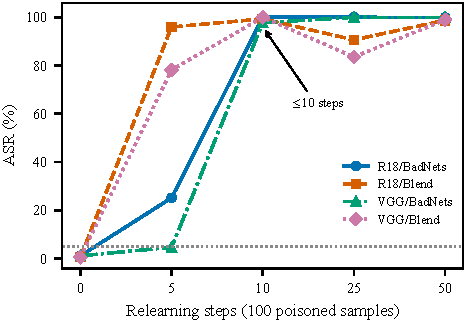
\includegraphics[width=\columnwidth]{fig9_relearn.pdf}
\caption{ASR of the oracle-deleted gold model after $k$ gradient steps on one
hundred fresh poisoned samples. All four settings return to at least 97.6\% ASR
within ten steps.}
\label{fig:relearn}
\end{figure}

\subsection{What the Probes Can and Cannot Certify}
Fig.~\ref{fig:probes} places both probes on the same axis, the fraction of poison
removed. Panel (a) is the membership-inference AUC. It is at chance at every
fraction, including the fully poisoned model, so on these models it cannot
certify anything about poison: the probe never had a signal to lose. This matters
because an AUC near 0.5 is sometimes reported as evidence of successful
unlearning. Here it is evidence only that the training procedure leaves no
detectable membership trace, which was already true before removal. Panel (b) is
the KL divergence between the model's outputs on clean and trigger-stamped
inputs. It stays between 12.0 and 28.2 while any poison remains and falls to zero
only when every poisoned sample is removed. Unlike the membership probe, it
tracks the poison, but it certifies current behaviour rather than the absence of
the capability: at 100\% removal it reads zero on the same gold model that
relearns to 97.7\% ASR within ten steps.

\subsection{SISA}
SISA-5 is the strongest efficiency-oriented alternative in our suite: it removes
the backdoor at full recall, reaching ASR $3.04\%$ with clean accuracy
$70.38\%$. The clean accuracy is 18.3 points below the frozen gold model, so the
run fails the joint criterion by a wide margin. At recall 0.5 the ASR is
$100.00\%$ and the clean accuracy $67.49\%$: the method inherits the same recall
cliff as deletion, on top of its sharding cost. The pilot runs with ten and
twenty shards are worse still ($50.25\%$ clean at ASR $6.26\%$, and $37.59\%$ at
$8.04\%$), which is the expected direction: more shards mean less data per
constituent model and a larger utility penalty. SISA's guarantee is about the
data that is forgotten, not about the data that is missed, and it does not change
the cliff.

\subsection{Fine-Pruning}
Fine-pruning removes the filters with the smallest average activation on clean
data. On ResNet-18/BadNets, pruning 40\% of channels leaves ASR at $63.64\%$ and
clean accuracy at $65.50\%$; pruning 60\% reaches ASR $0.00\%$ with clean
accuracy $61.30\%$. On VGG-16-BN/BadNets the method needs 90\% of channels before
ASR falls to zero, at which point clean accuracy is $67.85\%$. The base models in
this block are weaker than the frozen gold (69.5\% and 71.0\% clean), because the
block was run under a shorter schedule, so the absolute numbers are not directly
comparable with Table~\ref{tab:e1grid}. The relative cost is: 8.2 points for
ResNet-18 and 3.1 points for VGG-16-BN from their own bases, plus the 18--19-point
gap between those bases and the frozen protocol. Fine-pruning is also
trigger-agnostic in the wrong sense: it can only remove a backdoor that is
visible as dormant neurons, and it has no mechanism for poison that is
distributed across the network.

\begin{figure}[!tb]
\centering
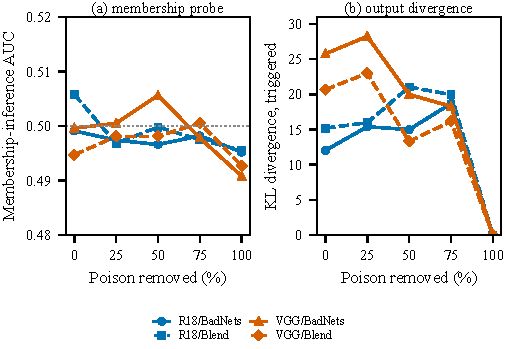
\includegraphics[width=\columnwidth]{fig18_durability_probes.pdf}
\caption{Representational probes on the E2 models as a function of the fraction
of poison removed. (a) Membership-inference AUC is at chance at every fraction,
including the fully poisoned model. (b) KL divergence between clean and
trigger-stamped outputs is high while any poison remains and zero only at full
removal. Neither probe distinguishes suppression from erasure.}
\label{fig:probes}
\end{figure}

\subsection{Pilot Baselines}
Table~\ref{tab:baselines} also lists rows from the earlier pilot protocol. They
are not pooled with the frozen results, and we mark them as pilot rows. Three of
them are informative. Partial deletion of 25\%, 50\%, or 75\% of the poison
leaves ASR between 99.86\% and 100.00\%, which is the same step seen in E2.
Gradient ascent in the pilot leaves ASR at 99.93\% on ResNet-18 and 99.99\% on
VGG-16-BN (mean 99.96\%), consistent with the normalisation artefact diagnosed
in Section~\ref{sec:calib}. Label repair without inoculation averaged ASR
$0.46\%$ at $83.37\%$ clean accuracy over two pilot runs (0.54\%/85.55\% on
ResNet-18 and 0.38\%/81.19\% on VGG-16-BN), a 6.6-point cost against that
protocol's approximately 90\% baseline. It did not reproduce under the frozen
protocol, where label repair alone gave $8.63$--$16.36\%$ ASR with clean accuracy
within 1.5 points. We report both, and we do not use the pilot row to support a
success claim.

\begin{table}[t]
\centering
\caption{Efficiency-oriented and sharded baselines.}
\label{tab:baselines}
\footnotesize
\begin{tabular}{lccc}
\toprule
\textbf{Method} & \textbf{Recall} & \textbf{Clean} & \textbf{ASR} \\
\midrule
SISA-5 (this protocol) & 1.0 & 70.38 & 3.04 \\
SISA-5 (this protocol) & 0.5 & 67.49 & 100.00 \\
SISA-5 (pilot) & oracle & 63.83 & 3.79 \\
SISA-10 (pilot) & oracle & 50.25 & 6.26 \\
SISA-20 (pilot) & oracle & 37.59 & 8.04 \\
Fine-pruning R18, 40\% & -- & 65.50 & 63.64 \\
Fine-pruning R18, 60\% & -- & 61.30 & 0.00 \\
Fine-pruning VGG, 90\% & -- & 67.85 & 0.00 \\
\midrule
Gradient ascent (pilot) & -- & 87.62 & 99.96 \\
Label repair FT (pilot) & -- & 83.37 & 0.46 \\
Partial deletion 25\% (pilot) & -- & 89.97 & 99.98 \\
Partial deletion 50\% (pilot) & -- & 90.13 & 99.96 \\
Partial deletion 75\% (pilot) & -- & 90.08 & 99.96 \\
\bottomrule
\end{tabular}
\par\vspace{1pt}\footnotesize\raggedright Reviewer-facing baselines. SISA and fine-pruning rows are measured; pilot rows use the minor project's earlier protocol (clean accuracy $\approx$90\%) and are shown for completeness, not pooled with the frozen results. Pilot values are means over the runs recorded in the master results table (two architecture variants for SISA and repair, four runs for partial deletion). SISA's clean accuracy is 18 points below the frozen gold model already at $r{=}1$; fine-pruning needs 60\% (ResNet) or 90\% (VGG) of channels pruned before ASR falls, by which point clean accuracy has dropped 8 and 3 points respectively.
\end{table}


\subsection{Summary of the Baselines}
The baselines divide into two groups. Methods that delete data and retrain
(SISA, deletion) can remove the backdoor at full recall, but they pay a utility
cost that ranges from 18 points for SISA-5 to a fraction of a point for deletion,
and they inherit the recall cliff. Methods that edit the model without a
trigger-aware objective (fine-pruning, gradient ascent, retain fine-tuning) either
need to remove most of the network or do not remove the backdoor at all. None of
them reaches the joint criterion at a cost below retraining with full recall. The
recipe is the only method that reaches it at recall 0.5, and it does so with
trigger knowledge that the baselines do not require.
